\documentclass{article}
\usepackage[utf8]{inputenc}
\usepackage[margin=1in]{geometry}
\usepackage{scrextend}
\usepackage[dvipsnames]{xcolor}
\usepackage{hyperref}
\usepackage{amsmath}
\hypersetup{
    colorlinks=true,
    linkcolor=blue,
    filecolor=magenta,      
    urlcolor=blue,
}
\setlength\parindent{0pt}
\usepackage{setspace}
\usepackage{color}

\begin{document}

\begin{center}
{\LARGE EAPS First Year Course 2019}\\
\vspace{10pt}
{\Large Writing Resources at MIT}\\
\vspace{6pt}
\end{center}
Writing is an integral component of your PhD work. Below are some tips, instructions, and resources to help you write and cite everything from fellowship applications, to conference abstracts, to generals papers.

\section*{Typesetting}
First, \emph{where} will you write your words? In my experience, there are two primary options:
\textbf{Microsoft Word and \LaTeX}.
Your choice will affect how your writing is typeset and how your collaborators/editors/advisors provide feedback. MIT provides Microsoft Office (Word, Excel, Powerpoint, OneNote) to students free \href{https://ist.mit.edu/office/license}{at this link}. If you would like to download \LaTeX, there are a couple of options, but I recommend \href{https://pages.uoregon.edu/koch/texshop/}{TexShop}.\\

There are pros and cons to both word processing options: Word is probably more familiar to many of you, and arguably much easier to use. Many people prefer editing papers using Word, which allows for easy ``track changes'' and commenting. On the other hand, Latex is much better at typesetting equations\footnote{I have this very useful page bookmarked for easy access:\href{ https://en.wikibooks.org/wiki/LaTeX/Mathematics}{https://en.wikibooks.org/wiki/LaTeX/Mathematics}}, has a very straightforward way of referencing other (labeled) parts of the text, and allows you to customize your document to a level that I have never quite figured out in Word. 

\subsection*{Overleaf}
If you choose to write in Latex, MIT provides subscriptions to \href{https://www.overleaf.com}{Overleaf}, an online Latex editor. In addition to a more aesthetically pleasing interface than TexShop, Overleaf has many templates and compatibility with \href{https://www.sharelatex.com}{ShareLatex} and
\href{https://github.com}{GitHub}. By using Overleaf and GitHub together, you can easily edit the same document or project both on- and off-line. (If you're interested in learning how to do this, Google it or ask Julia.)

\section*{References}
Citation is an integral part of scientific writing that somehow always ends up taking longer than anticipated. Fortunately, there are a few tools that can help. Many researchers in EAPS use \href{https://libguides.mit.edu/cite-write/mendeley#s-lg-box-wrapper-18620527}{Mendeley}, a citation manager offered freely by the MIT Libraries. You can use Mendeley to store, organize, and export citations for PDFs. Noah Anderson (nanderso@) will give a Mendeley tutorial on 9/13/19 and you can email him with questions. If you are writing in Latex, you should export your bibliography as a BibTex \texttt{(.bib)} file. Talk to Julia if you have questions about adding your references in Latex -- it can be a pain. Another (less sleek) option is to manually add information about the papers you reference to a BibTex library. I use BibDesk  (Figure \ref{fig:bib}), which comes in the TexShop distribution. 

\begin{figure}[h!]
    \centering
    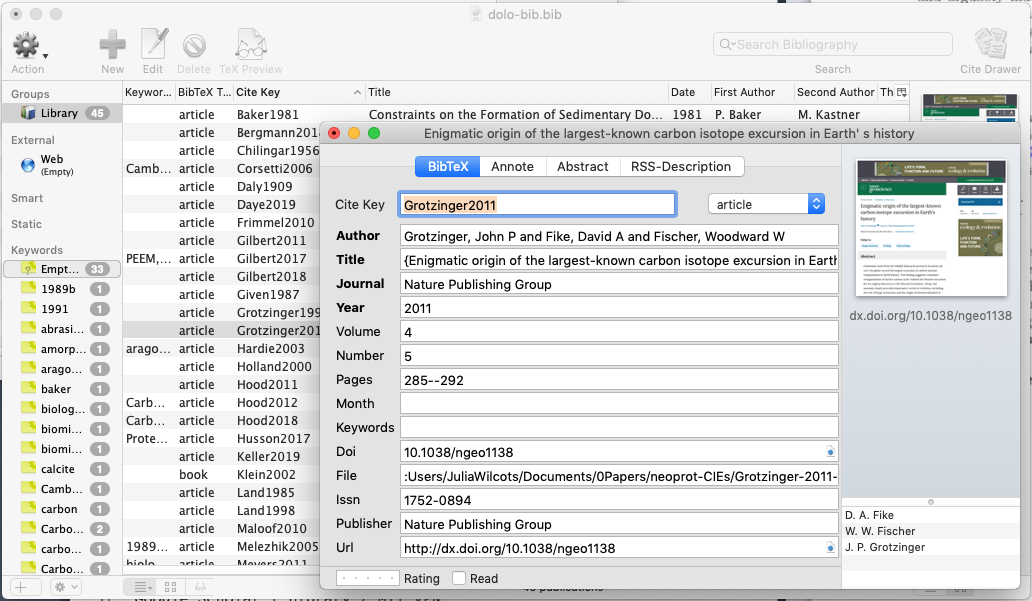
\includegraphics{bibdesk}
    \caption{Caption}
    \label{fig:bib}
\end{figure}


\subsection*{Finding papers}
Google Scholar + Library / MIT VPN

\section*{Figures}
We'll spend more time on this later... Adobe CD in HQ

\vspace{10pt}
\begin{labeling}{February 25 \hspace{1.5cm}}
\item [\textbf{February 11}] \textbf{Tyler}\\ A clumped isotope test for Neoproterozoic Snowball Earth deposits of NE Svalbard
\item [\textbf{February 19$\star$}] \textbf{Marjorie}\\Carbonates before skeletons: a database approach to the Precambrian carbonate record \\ $\star$Tuesday due to Monday holiday
\item [{\color{red}\textbf{February 21}}] {\color{red}\textbf{Special meeting - 10:00-11:00}\\ Read \href{https://brenhinkeller.github.io/files/GreatUnconformity2019.pdf}{Keller et al. 2019} and discuss with Perron group}
\item [\textbf{February 25}]
\item [\color{violet}\textbf{March 4}] {\color{violet} Read/discuss} \href{http://www.blakedyer.com/papers/Dyer2018.pdf}{Dyer et al. 2018} {\color{violet}for writing and figures}\\Or, {\color{MidnightBlue}Figure review: Tyler, Marjorie, Noah}
\item [\textbf{March 11}] \textbf{Adam}\\Carbonate clumped isotopes from Marinoan-age low latitude carbonates
\item [\textbf{March 18}] \textbf{Sam}\\Preservation and fidelity of climate proxy records in early Paleozoic carbonates
\item [\color{ForestGreen}\textbf{March 25}] {\color{ForestGreen} Spring break one day writing retreat for those who are here and interested}\\{\color{MidnightBlue} bring a figure}, peer review, {\color{BurntOrange}writing strategies}
\item [\textbf{April 1}] \textbf{Julia} \\
Dolomite!
\item [\textbf{April 8}] \textbf{Noah}\\Ooids!
\item [\textbf{April 17}] \textbf{Jocelyn}\\
\item [\textbf{April 22}] \textbf{Zahra}\\Clumped isotope paleothermometry of the Bitter Springs Stage in Svalbard: A case for solid-state reordering in the region?
\item [\textbf{April 29}] \textbf{Athena}\\Iron Formation!
\item [\textbf{May 6}] \textbf{Kristin} \\ Oman stratigraphy
\item [\color{red}\textbf{May 13}] {\color{red}TBD}
\item [\color{red}\textbf{May 20}] {\color{red}TBD}
\end{labeling}


\end{document}

